\documentclass[sigconf,review]{acmart}

\usepackage{amsmath}
\usepackage{booktabs}
\usepackage{placeins}
\usepackage{tabularx}
\usepackage{iftex}
\ifXeTeX
  \makeatletter
  \@ifpackageloaded{fontspec}{}{\usepackage{fontspec}}
  \makeatother
  \usepackage{xeCJK}
  \xeCJKsetup{CJKspace=true}
  \defaultfontfeatures{Ligatures=TeX}
  \IfFontExistsTF{TeX Gyre Termes}{%
    \setmainfont{TeX Gyre Termes}%
  }{%
    \IfFontExistsTF{Times New Roman}{%
      \setmainfont{Times New Roman}%
    }{%
      \setmainfont{STIX Two Text}%
    }%
  }
  \IfFontExistsTF{NanumBarunGothicOTF}{%
    \setCJKmainfont[
      ItalicFont={NanumBarunGothicOTF},
      SmallCapsFont={NanumBarunGothicOTF}
    ]{NanumBarunGothicOTF}%
    \setCJKsansfont{NanumBarunGothicOTF}%
    \setCJKmonofont{NanumBarunGothicOTF}%
  }{%
    \IfFontExistsTF{Noto Sans CJK KR}{%
      \setCJKmainfont[
        ItalicFont={Noto Sans CJK KR},
        SmallCapsFont={Noto Sans CJK KR}
      ]{Noto Sans CJK KR}%
      \setCJKsansfont{Noto Sans CJK KR}%
      \setCJKmonofont{Noto Sans CJK KR}%
    }{%
      \setCJKmainfont[
        Scale=0.92,
        ItalicFont={Apple SD Gothic Neo},
        SmallCapsFont={Apple SD Gothic Neo}
      ]{Apple SD Gothic Neo}%
      \setCJKsansfont[Scale=0.92]{Apple SD Gothic Neo}%
      \setCJKmonofont[Scale=0.92]{Apple SD Gothic Neo}%
    }%
  }
  \xeCJKDeclareCharClass{Default}{"00B7}
\else
  \usepackage{kotex}
\fi

\newif\ifanonymoussubmission
\ifdefined\ANONBUILD
  \anonymoussubmissiontrue
\else
  \anonymoussubmissionfalse
\fi

\newcommand{\system}{TRACE-RPG}
\newcommand{\Valid}{\mathrm{valid}}
\newcommand{\AcceptSet}{\mathcal{A}}
\newcommand{\GoalSet}{\mathcal{G}}
\newcommand{\HitSet}{\mathcal{H}}
\newcommand{\SchemaSet}{\mathcal{S}}
\newcommand{\RepoURL}{\ifanonymoussubmission [Anonymous Repository URL withheld for double-anonymous review]\else \url{https://github.com/akillness/neural_symbolic_in_game}\fi}
\AtBeginDocument{\emergencystretch=2.5em}
\providecommand{\Description}[2][]{}

\anonymoussubmissionfalse

\setcopyright{none}
\acmConference[FDG '27]{Foundations of Digital Games (Korean Companion)}{2027}{Seoul, Republic of Korea}

\begin{document}

\title{TRACE-RPG: 대화형 게임을 위한 감사 가능한 제안--커밋 경계와 결정론적 엔진 검증}

\author{정장영}
\affiliation{\institution{홍익대학교 게임학과}\city{서울}\country{대한민국}}
\author{강신진}
\authornote{교신저자.}
\affiliation{\institution{홍익대학교}\city{서울}\country{대한민국}}

\begin{abstract}
스키마에 부합하는 게임 내 행동 제안이라도 접근 불가 물체 요구, 비인가 전이, 조기 비밀 공개를 포함할 수 있다. \system{}는 Godot~4.7.1과 통합된 결정론적 7술어 게이트, 반례 유도 수리 $\rho$, 해시 연결 리플레이로 제안·커밋 권한을 분리한다(정리 1--4). 1,664건 유한 그래프 감사에서 위험 커밋 260/416 $\rightarrow$ 0/416(수리 128/260), 5개 퀘스트 월드 120건 다중 홉 폐쇄에서 100.0\% 대 평면 50.83\%($p{<}10^{-16}$)를 달성하였다. 특히 16개 라이브 Gemini $\rightarrow$ 헤드리스 Godot~4.7.1 폐루프 에피소드(+ 0-LLM 독립 재실행 16회)에서 위험 커밋·비밀 유출 0/16과 16/16 재실행 일치를 기록했으며(Hydrogen 8/8 \texttt{EXACT\_}\allowbreak\texttt{TERMINAL\_}\allowbreak\texttt{HASH}; Flash 5/8, 파싱실패 4 보존 및 엄격 액터 ID 안전 거부 1건), 30에피소드 5암 실딩(66.7\% 대 33.3\%, $p{=}0.00195$), 60작업 라이브 비교($\rho$ 12/12 대 LLM 자가수리 2/12), 268건 한·영 우회 검증(재현율 97.2--100.0\%, FRR 0/72)과 \texttt{TR01--TR06} 패킷(\texttt{AWAITING\_}\allowbreak\texttt{HUMAN\_}\allowbreak\texttt{RATERS})을 보고한다.
\end{abstract}

\begin{CCSXML}
<ccs2012>
   <concept>
       <concept_id>10010147.10010178.10010187</concept_id>
       <concept_desc>Computing methodologies~Knowledge representation and reasoning</concept_desc>
       <concept_significance>500</concept_significance>
   </concept>
   <concept>
       <concept_id>10011007.10011074.10011099</concept_id>
       <concept_desc>Software and its engineering~Software verification and validation</concept_desc>
       <concept_significance>300</concept_significance>
   </concept>
</ccs2012>
\end{CCSXML}

\ccsdesc[500]{Computing methodologies~Knowledge representation and reasoning}
\ccsdesc[300]{Software and its engineering~Software verification and validation}

\keywords{게임 인공지능, 인터랙티브 내러티브, 뉴로심볼릭 시스템, Godot, 결정론적 검증}

\maketitle

\section{서론}
스키마에 부합하는 게임 내 행동 제안이라도 접근할 수 없는 물체를 요구하거나 권한이 없는 상태 전이, 혹은 현재 시점에서 공개할 수 없는 비밀 발화를 포함할 수 있다. 서사적 정합성(grounding)과 개연성 있는 대화 생성 \cite{S03_weir2024ontologically,S20_ashby2023personalized}은 후보 콘텐츠를 제공할 뿐이며, 게임 엔진은 현재 상태에서 어떤 전이를 승인할지 별도로 판정해야 한다.

\system{}는 이 판정을 외부의 제안--커밋(proposal-to-commit) 경계에서 강제한다(그림~\ref{fig:architecture}). 모델과 어댑터가 구조화된 후보를 제출하면 결정론적 게이트가 행동 정책, 선행조건, 물체 도달 가능성, NPC 지식, 정보 공개 권한, 효과, 퀘스트 단계 단조성을 검사한다. 검사에 실패하면 게이트는 제한된 수리를 위한 구조화된 오류를 반환하며, 수리는 정본 상태(canonical state)가 아닌 후보만 수정하고 동일 상태 재검증을 통과한 경우에만 상태를 갱신한다. 여덟 역할 읽기 전용 온톨로지 뷰는 쓰기 권한 없이 출처 선언과 검사·결정을 연결하며, 해시 연결 전이 기록은 의미적 리플레이와 배정 전수 회계(assignment-complete accounting)를 보장한다.

개념적으로 이 계약은 단순 사실 일치(factual grounding)를 넘어 NPC의 \emph{인식론적 지식 경계}(행위자가 알고 있는 사실)와 \emph{정보 공개 권한 정책}(현재 퀘스트 단계에서 발화할 수 있는 사실)을 분리한다. 방법론적으로는 LLM 호출이 0회인 결정론적 검증 계층(게이트 검사, 유도 수리, 엔진 리플레이)과 실패를 누락 없이 보존하는 제한된 확률적 제안기 계층을 엄격히 분리한다.

결정론적 감사에서 스키마 전용 대조군은 32개 유한 그래프 조합에 걸쳐 기준상 무효인 제안 260/416건을 커밋한 반면, 모든 의미 게이트 조건은 0/416건을 기록했고 최초 유효 제안 156/156건(오탐 0/156) 및 고유 구조 서명 11/11종을 모두 보존했다. 반례 유도 수리는 최초 무효 제안 260건 중 128건을 유효 커밋으로 복구했다. 단일 홉 정보 공개 검사에서도 일반 규칙과 온톨로지 게이트는 60/60건 일치하며 위험 공개 51건을 차단했고, 후속 48건 다중 홉 폐쇄 벤치마크에서는 양자를 뚜렷이 구분한다(\texttt{ontology\_}\allowbreak\texttt{multihop\_}\allowbreak\texttt{gate} 48/48 대 \texttt{flat\_}\allowbreak\texttt{1hop\_}\allowbreak\texttt{rule} 20/48, 위험 누출 28건 차단). 여기에 확장 0-LLM 감사, 불변식 \textbf{I1--I4}에 대한 형식 정리 1--4, 24에피소드 라이브 다중 퀘스트 Gemini 평가(2종 모델, 3개 월드, 위험 커밋 0건, 엄격 리플레이 24/24), 2차 한·영 우회 검증기(우회 재현율 97.2\% 및 양성 오거부 0.0\%), 그리고 실제 트레이스 결속 36항목 블라인드 인간 평가 패킷(\texttt{AWAITING\_}\allowbreak\texttt{HUMAN\_}\allowbreak\texttt{RATERS})과 Croissant~1.0 메타데이터를 더해 재현 가능한 공개 경계를 완성한다.

\section{관련 연구와 연구 공백}
정합성, 기억, 계획, 역할 기반 에이전트 \cite{S03_weir2024ontologically,S20_ashby2023personalized,S07_park2023generative,S08_shao2023character} 및 플레이어·대화 시스템 \cite{S21_akoury2023player,S22_hochreiter2026beyond,S23_yin2026contextualized,S02_figueiredo2025scaffolded}은 맥락적 상호작용을 지원하는 반면, 본 연구는 인코딩된 현재 상태와 공개 정책이 제안된 전이를 허용하는지를 판정한다. 정서 및 몰입 모델링 \cite{S24_yannakakis2011experiencedriven,S25_melhart2020engagement,S26_wang2026engagement}은 생성 스타일을 안내할 뿐 상태 변경 권한을 부여하지 않는다.

기존 벤치마크와 자동 플레이테스팅은 상태, 체화 환경, 콘텐츠, 과정, 사회적 상호작용, 장기 과업을 다루며 \cite{S11_cote2019textworld,S12_wang2022scienceworld,S13_fan2022minedojo,S14_perezliebana2019gvgai,S15_liu2024agentbench,S16_ma2024agentboard,S17_zhou2024sotopia,S18_paglieri2025balrog,S19_lepelletier2022playtesting}, NCP-Bench는 서사적 일관성과 사실 정합성을 평가한다 \cite{S58_ma2026ncpbench}. 문법·스키마·어포던스·규칙 기반 기법 \cite{S09_geng2023grammar,S10_beurerkellner2023prompting,S36_scholak2021picard,S50_kambhampati2024llmmodulo,S51_ichter2023saycan,S52_wang2025agentspec,S53_li2025settingdc,S54_zhou2025story2game,S42_buongiorno2024pangea}, 반례 기반 수리 \cite{S45_madaan2023selfrefine,S48_shinn2023reflexion,S46_chen2023selfdebug,S47_solarlezama2006sketching}, 재현성·리플레이 표준 \cite{S31_agarwal2021precipice,S33_pineau2021reproducibility,S56_feng2025agentrr,S59_sun2025bdc}이 본 설계의 토대다. 스키마 적합성과 행위 합법성, 또는 사실 정합성과 발화 안전성을 동일시하던 선행 연구와 달리, \system{}는 스키마 파싱, 인식론적 지식, 공개 권한, 정본 상태 커밋을 독립 감사 가능한 게이트로 분리한다.


\begin{figure*}[!t]
  \centering
  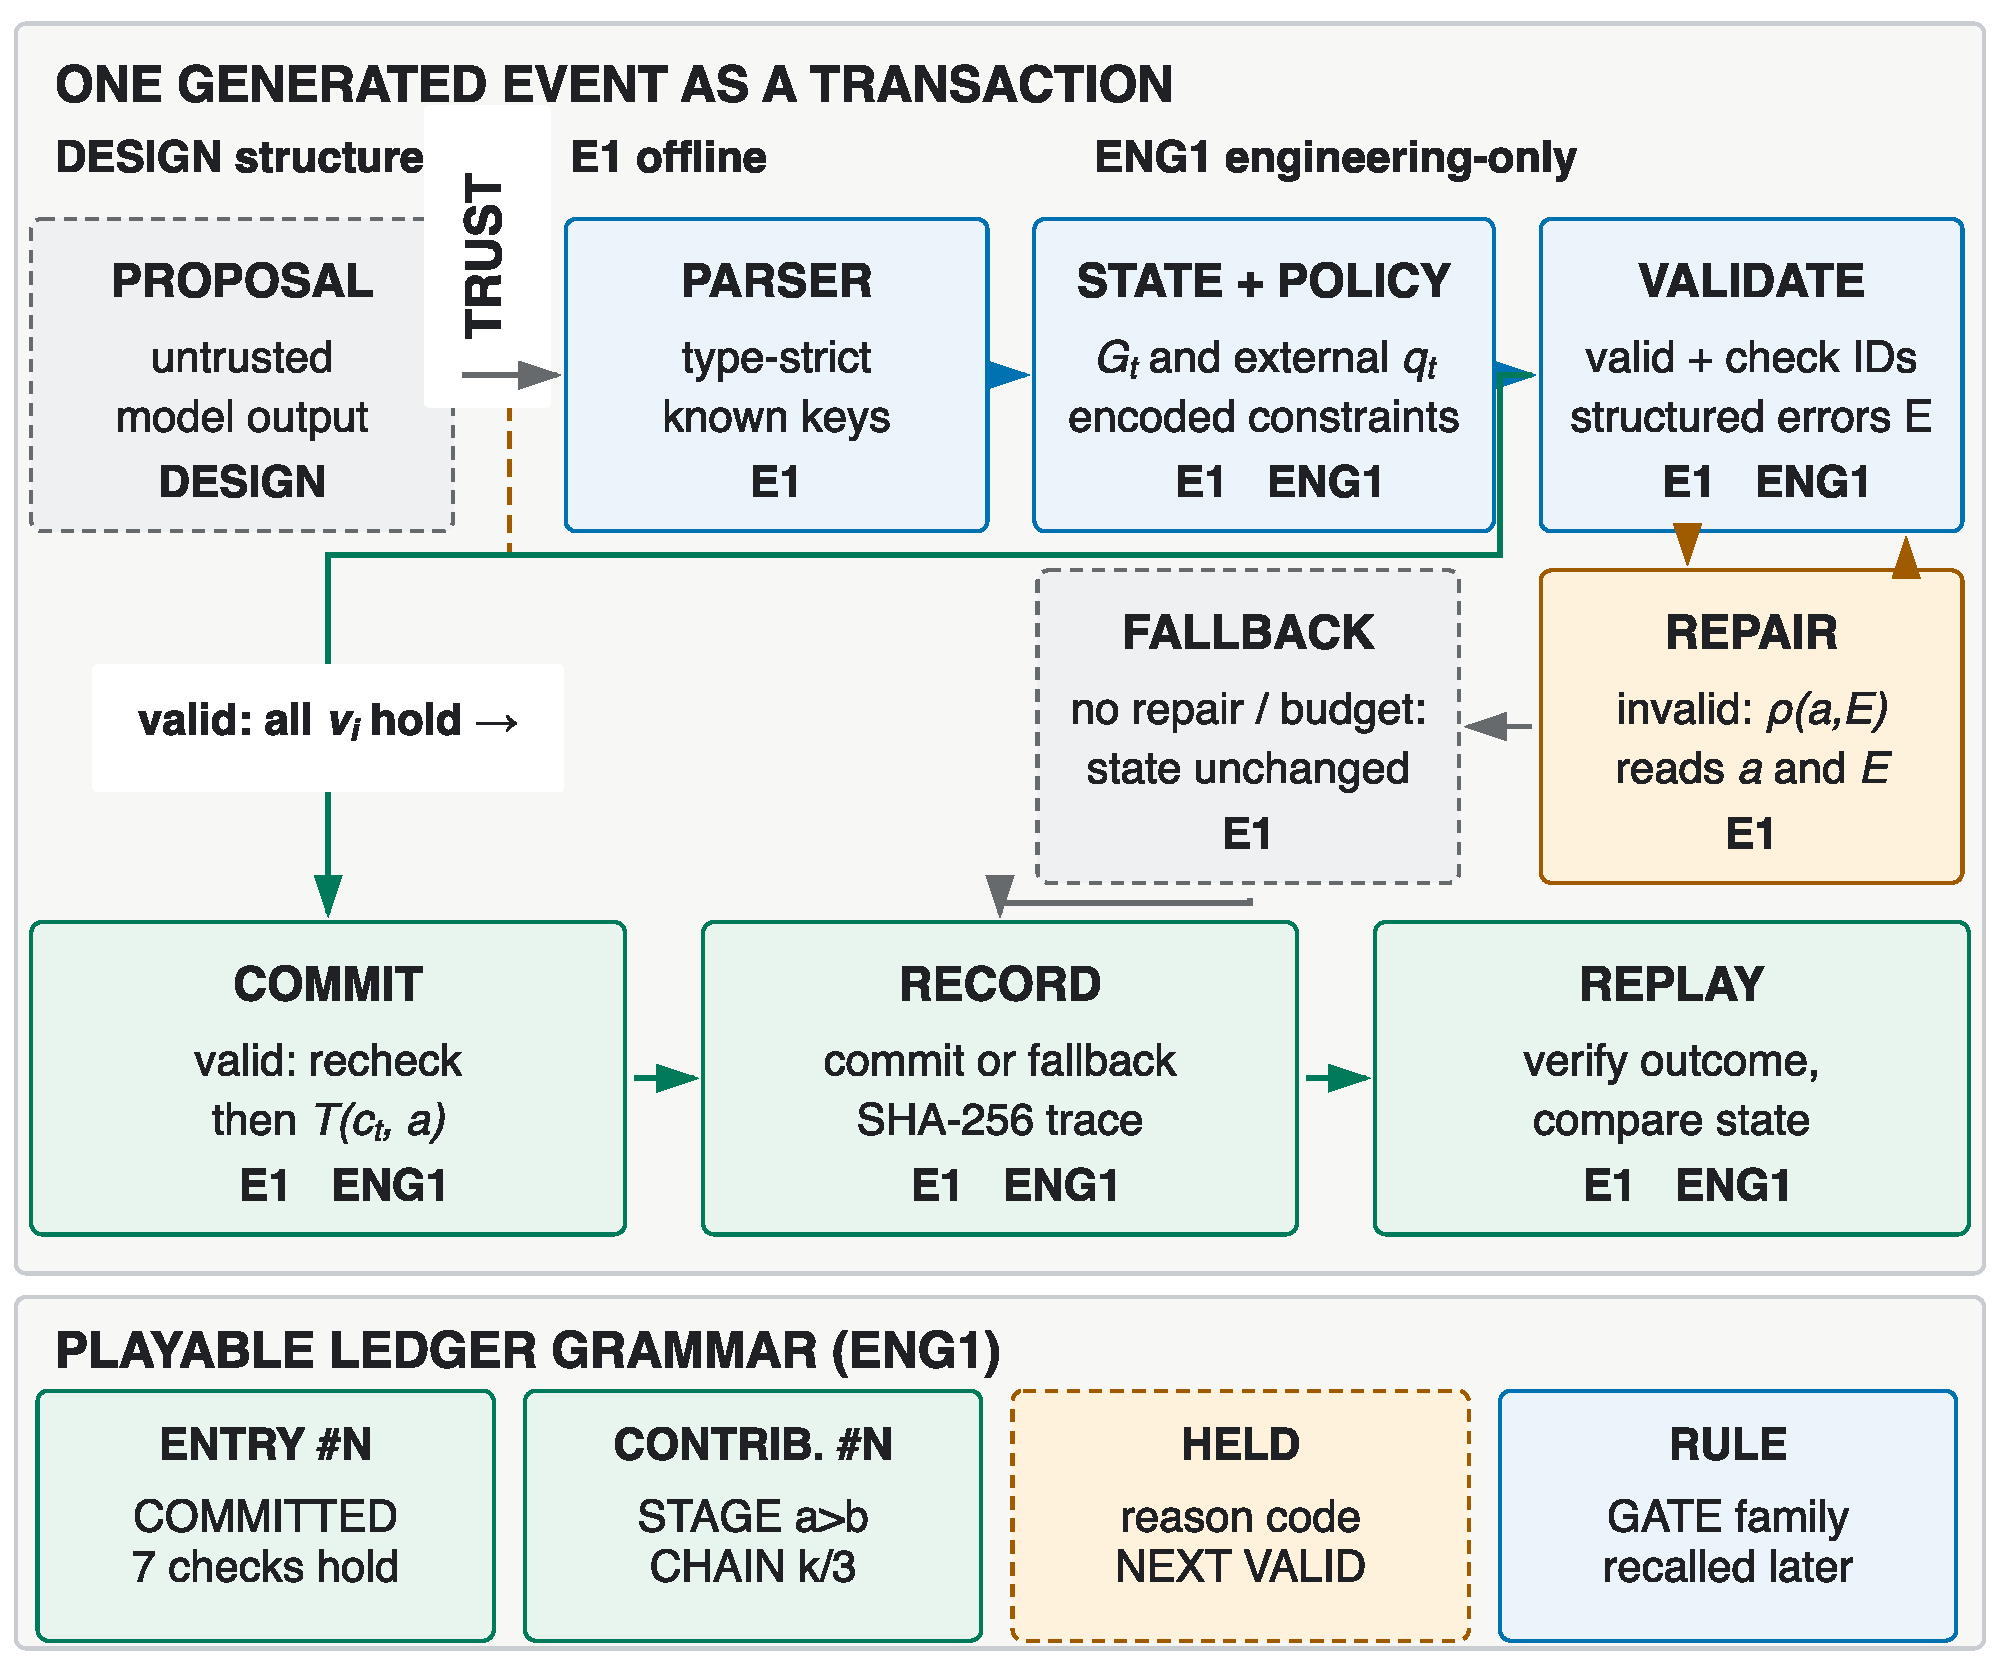
\includegraphics[width=0.72\textwidth]{../../figures/fig_architecture.pdf}
  \caption{정책과 상태 $c_t$가 제안을 게이팅하며, 오류는 $\rho$ 수리 또는 상태 불변 fallback으로 이어진 뒤 재검증을 거쳐 커밋된다.}
  \Description{제안 제출, 7술어 결정론적 검증, 제한적 수리, 재검증 및 커밋 원장을 보여주는 아키텍처 다이어그램.}
  \label{fig:architecture}
\end{figure*}

\section{문제 정의와 보장 경계}\label{sec:problem}
입력 $c_t=(G_t,q_t)$에서 $G_t$는 형식이 지정된 게임 스냅샷(장소, 도달 가능 위치, 물체 배치, 소지품, 사실, NPC 지식, 퀘스트 단계)을, $q_t$는 외부에서 저작된 행동 정책·정보 공개·퀘스트 단계 제약을 나타낸다. 검증 술어는 직전 이력 $h_{<t}$를 역산하거나 $q_t$를 변경하지 않으며, 검색 결과나 정서 점수는 쓰기 권한이 없다.

비신뢰 제안 $a_t$를 엄격히 파싱한 뒤, 검증기는 7개의 결정론적 술어를 실행하여 \texttt{ValidationResult}(\allowbreak$\mathrm{valid},E_t,C_{\mathrm{run}}$)를 반환한다:
\begin{equation}
\begin{aligned}
V(c_t,a_t)&=(\mathrm{valid},E_t,C_{\mathrm{run}}),\\
\boldsymbol{v}&=(v_{\mathrm{policy}},v_{\mathrm{pre}},v_{\mathrm{reach}},\\
&\qquad v_{\mathrm{know}},v_{\mathrm{disc}},v_{\mathrm{elig}},v_{\mathrm{stage}})\in\{0,1\}^{7},
\end{aligned}
\end{equation}
여기서 $\mathrm{valid}\equiv\bigwedge_{i=1}^{7}(v_i=1)$이며, $E_t$는 오류 코드·개체·원인·수리 힌트를 기록한다. 정본 상태는 7개 술어를 모두 통과한 경우에만 갱신된다:
\begin{equation}
c_{t+1}=\begin{cases}
T(c_t,a_t), & \bigwedge_{i=1}^{7}(v_i=1),\\
c_t, & \text{otherwise.}
\end{cases}
\label{eq:transition}
\end{equation}

\subsection{스키마 유효성, 권한, 목표 달성의 분리}\label{sec:authorization-sets}
행동 전 상태 $c_t$, 저작 정책, 엄격 스키마를 고정하고 스키마 유효 후보 집합을 $\SchemaSet$라 할 때, 권한과 목표 달성을 다음과 같이 분리한다:
\begin{equation}
\begin{aligned}
\AcceptSet(c_t)&=\{a\in\SchemaSet:V(c_t,a).\mathrm{valid}\},\\
\GoalSet(c_t)&=\{a\in\SchemaSet:\operatorname{Goal}(T(c_t,a))\},\\
\HitSet(c_t)&=\AcceptSet(c_t)\cap\GoalSet(c_t)\subseteq\AcceptSet(c_t)\subseteq\SchemaSet.
\end{aligned}
\end{equation}
금지 사실을 선언한 스키마 유효 후보는 $\AcceptSet$ 밖에 놓이며, 허용된 관찰 행동은 $\AcceptSet$에 속하지만 $\GoalSet$ 밖에 놓일 수 있다. 지식과 공개 권한은 독립 입력이다. 예컨대 NPC는 0단계와 1단계 모두에서 \texttt{keeper\_\allowbreak secret}을 알고 있으나, 공개는 0단계에서 금지되고 1단계에서 허용된다.

\subsection{불변식 I1--I4에 대한 형식 안전성 정리}\label{sec:formal-proofs}
결정론적 전이 규칙(식~\eqref{eq:transition})과 엄격 파서 \texttt{parse\_}\allowbreak\texttt{candidate\_}\allowbreak\texttt{mapping} 아래에서 불변식 \textbf{I1--I4}는 임의의 유한 인코딩 상태 $c_t=(G_t,q_t)$, 수리 예산 $K\in\mathbb{Z}_{\geq 0}$ 및 정상 반환 콜백에 대한 조건부 구조 정리로 성립한다.

\noindent\textbf{정리 1 (I1: 상태 보존 안전성).} \emph{초기 후보가 엄격 파싱을 통과하지 못하거나 $K{+}1$회 모든 시도에서 $V(c_t,a^{(j)}).\mathrm{valid}=\mathrm{false}$이면 $c_{t+1}=c_t$이며 커밋된 효과는 비어 있다.}
\par\noindent\textit{증명.} \texttt{parse\_}\allowbreak\texttt{candidate\_}\allowbreak\texttt{mapping}은 커밋 전에 비정형 제안을 거부하며, 그림~\ref{alg:commit}에서 $\operatorname{Commit}$은 $\mathrm{ok}=\mathrm{true}$일 때만 도달 가능하고 $j=K$에서는 $\operatorname{Fallback}(c_t)$이 식~\eqref{eq:transition}에 의해 $c_t$를 그대로 반환한다. \hfill$\square$

\noindent\textbf{정리 2 (I2: 유한 종료와 상태 비참조 세탁 방지 수리).} \emph{유한 $K{\geq}0$과 정상 반환 콜백 하에서 루프는 $V$를 최대 $K{+}1$회 호출하며, 상태 변경 직전 $V(c_t,a^{(j)})$를 재검증하고, $\rho$는 \texttt{WorldState} 의존 권한 오류 클래스를 변경하지 않는다.}
{\sloppy\par\noindent\textit{증명.} 계수기 $j$는 $0$에서 시작하여 증가 전 $j=K$를 검사하므로 $V$ 호출은 최대 $K{+}1$회로 유계다. 표~\ref{tab:rho-rules}에 따라 $\rho(a,E)$는 \texttt{WorldState}를 읽지 않고 $(a,E)$만 입력받아 \texttt{UNKNOWN\_}\allowbreak\texttt{ACTION\_}\allowbreak\texttt{TYPE}, \texttt{UNREACHABLE\_}\allowbreak\texttt{REQUIRED\_}\allowbreak\texttt{OBJECT}, \texttt{NPC\_}\allowbreak\texttt{KNOWLEDGE\_}\allowbreak\texttt{VIOLATION}, \texttt{NPC\_}\allowbreak\texttt{DIS\-CLOSURE\_}\allowbreak\texttt{KNOW\-LEDGE\_}\allowbreak\texttt{VIO\-LATION}, \texttt{FORBIDDEN\_}\allowbreak\texttt{DISCLOSURE}, \texttt{QUEST\_}\allowbreak\texttt{STAGE\_}\allowbreak\texttt{VIOLATION}, \texttt{QUEST\_}\allowbreak\texttt{STAGE\_}\allowbreak\texttt{REGRESSION}을 항등 사상으로 두고 동일 필드 상충 편집을 제거한다. \hfill$\square$\par}

\noindent\textbf{정리 3 (I3: 정책 유계 상태 변이).} \emph{커밋된 모든 전이는 7개 술어 $v_1\dots v_7$을 만족하며 \texttt{ActionPolicy.}\allowbreak\texttt{allowed\_}\allowbreak\texttt{effects}에 허용된 효과만 반영한다.}
\par\noindent\textit{증명.} 엄격 파서가 12개 \texttt{CANDIDATE\_}\allowbreak\texttt{FIELDS}를 동결하고, $v_{\mathrm{policy}}{=}1$이 허용 집합 포함 여부를 검증하며, $T$는 선언 외 키를 기록하지 않는다. \hfill$\square$

\noindent\textbf{정리 4 (I4: 결정론적 의미 리플레이 및 변조 탐지).} \emph{\texttt{allow\_}\allowbreak\texttt{defaults=}\allowbreak\texttt{false} 파싱과 동결 $(V,T)$ 하에서 정렬된 해시 연쇄 전이 기록을 $c_0$부터 재실행하면 $c_T$가 유일하게 복원되며 단일 단계 변조도 SHA-256 연쇄 불일치로 탐지된다.}
\par\noindent\textit{증명.} $V,T$는 $(c_t,a_t)$의 순수 결정론적 함수이고 각 기록은 $(\mathrm{hash}(c_t),\allowbreak a_t,\allowbreak V(c_t,a_t),\allowbreak\mathrm{hash}(c_{t+1}))$을 해싱하므로 귀납적으로 $\mathrm{hash}(c'_T)=\mathrm{hash}(c_T)$가 일치한다. \hfill$\square$

\section{TRACE-RPG 아키텍처와 알고리즘}\label{sec:arch}
모델과 어댑터가 후보 행동을 제안하면 엄격 파서가 미등록 키와 모호한 타입을 거부하고, 버전 관리 브리지가 관측·제안·검증·거부·대체(fallback)·커밋을 전달한다(그림~\ref{fig:architecture}, 표~\ref{tab:validators}). 여덟 역할 읽기 전용 온톨로지 뷰(\texttt{World}, \texttt{Actor}, \texttt{Knowledge}, \texttt{Fact}, \texttt{Policy}, \texttt{Quest}, \texttt{Action}, \texttt{Trace})는 쓰기 권한 없이 출처 선언을 실행 검사 및 리플레이 영수증에 연결한다.

\begin{table}[!tbp]
\caption{인코딩된 7술어 검증기 경계}
\label{tab:validators}
\centering
\footnotesize
\begin{tabularx}{\columnwidth}{@{}>{\raggedright\arraybackslash}p{0.25\columnwidth}>{\raggedright\arraybackslash}X>{\raggedright\arraybackslash}p{0.16\columnwidth}@{}}
\toprule
\textbf{술어} & \textbf{거부 조건} & \textbf{실패 시} \\
\midrule
행동 정책 & 미등록 행동/유형, 필수 조건·효과 누락, 비허용 효과 & 상태 불변 \\
선행조건 & 부재 또는 거짓인 필수 조건 & 상태 불변 \\
도달 가능성 & 접근 불가능한 대상 물체 & 상태 불변 \\
NPC 지식 & 행위자 지식에 없는 사실 사용·공개 & 상태 불변 \\
정보 공개 & 선언된 금지 사실 포함 & 상태 불변 \\
퀘스트 단계 & 현재 단계보다 높은 요구 단계 & 상태 불변 \\
단계 단조성 & 역행하는 퀘스트 단계 전이 & 상태 불변 \\
\bottomrule
\end{tabularx}
\end{table}

\begin{figure}[!tbp]
\centering
\footnotesize
\begin{tabular}{@{}rl@{}}
1: & $a\leftarrow\operatorname{Propose}(c)$; $j\leftarrow0$ \\
2: & \textbf{repeat} \\
3: & \quad $(\mathrm{ok},E)\leftarrow V(c,a)$; $\operatorname{Record}(a,E)$ \\
4: & \quad \textbf{if} $\mathrm{ok}$ \textbf{then assert} $V(c,a).\mathrm{ok}$; \textbf{return} $\operatorname{Commit}(c,a)$ \\
5: & \quad \textbf{if} $j=K$ \textbf{then return} $\operatorname{Fallback}(c)$ \\
6: & \quad $a\leftarrow\operatorname{Repair}(c,a,E)$; $j\leftarrow j+1$ \\
7: & \textbf{until terminal}
\end{tabular}
\caption{검증--수리--커밋 루프는 최대 $K+1$회 시도를 기록하고 커밋 직전에 재검증한다.}
\Description{최대 K+1회 시도를 기록하고 커밋 직전 재검증하는 검증-수리-커밋 루프 의사코드.}
\label{alg:commit}
\end{figure}

유도 수리 연산자 $\rho(a,E)=a\oplus\bigcup_{e\in E}\delta(e)$(그림~\ref{alg:commit}, 표~\ref{tab:rho-rules})는 \texttt{WorldState}를 전혀 읽지 않고 후보 $a$와 구조 오류 $E$만 입력받아 도달 가능성·지식·공개 위반의 우회 세탁(state laundering)을 차단한다. 전이 기록은 이전 상태, 후보, 검증 결과, 재계산된 최종 상태에 대해 비키(unkeyed) SHA-256 해시를 연쇄 기록하여 결정론적 의미 리플레이와 배정 전수 분모 계수를 지원한다.

\begin{table}[!tbp]
\caption{유도 수리 연산자 $\rho(a,E)$의 오류 유형별 편집 규칙}
\label{tab:rho-rules}
\centering
\footnotesize
\begin{tabularx}{\columnwidth}{@{}>{\raggedright\arraybackslash}X>{\raggedright\arraybackslash}X@{}}
\toprule
\textbf{검증기 오류 유형} & \textbf{후보 $a$에 대한 편집 $\delta(e)$} \\
\midrule
정책 선행조건 / 효과 누락 & 명시된 술어 또는 효과 삽입 \\
정책 효과 위반 & 비허용 효과 제거 \\
불만족 선행조건 & 명시된 술어 제거 \\
비인가 단계 변경 & \texttt{quest\_stage\_effect} 초기화 \\
미등록 행동; 도달·지식·공개·단계 오류 & 무연산(no-op, 상태 세탁 방지) \\
\bottomrule
\end{tabularx}
\end{table}

\section{평가}\label{sec:eval}
0-LLM 결정론적 감사 계층과 제한된 확률적 제안기 파일럿을 분리 보고하며, 서로 다른 코호트와 분모는 통합하지 않는다.

\subsection{E1 오프라인 적합성 및 결정론적 경계 감사}
\textbf{E1}(게이트 픽스처 13건, 조건당 수리 12건)에서 네 조건 모두 구성 불변식(게이트 13/13, 무결성 결함 10/10)을 만족했다. 무효 수리 사례에서는 \texttt{rejection\_only}와 \texttt{unchanged\_retry}가 0/12, \texttt{WorldState}를 읽지 않는 유도 수리 $\rho$가 5/12, 상태 참조 오라클이 6/12를 복구했다.

단일 월드 픽스처를 넘어 권한 경계를 시험하기 위해, 방 개수(4, 8), 위상(잠긴 연쇄, 우회 분기), 열쇠 배치(4종), 퀘스트 단계(2종)를 교차한 32개 조합에 후보 13종을 적용해 조건당 416건(총 1,664건)과 표면 센티넬 48건(조건당 12건)을 평가했다.

\begin{table}[!tbp]
\caption{결정론적 권한 경계 감사 (조건당 416건 + 표면 센티넬 48건; 0 LLM 호출)}
\label{tab:boundary-full}
\centering
\footnotesize
\begin{tabularx}{\columnwidth}{@{}>{\raggedright\arraybackslash}X*{4}{>{\centering\arraybackslash}p{0.11\columnwidth}}@{}}
\toprule
\textbf{결과 (416/조건)} & \textbf{스키마} & \textbf{거부} & \textbf{재시도} & \textbf{유도 $\rho$} \\
\midrule
최초 무효 제안 & 260 & 260 & 260 & 260 \\
위험 최종 커밋 & 260 & \textbf{0} & \textbf{0} & \textbf{0} \\
수리 복구 (무효$\rightarrow$유효) & 0 & 0 & 0 & \textbf{128} \\
보류 (상태 불변) & 0 & 260 & 260 & 132 \\
목표 달성 & 124 & 124 & 124 & \textbf{252} \\
최초 유효 보존 (156건) & 156 & 156 & 156 & 156 \\
구조 서명 보존 (11종) & 11/11 & 11/11 & 11/11 & 11/11 \\
\bottomrule
\end{tabularx}
\end{table}

표~\ref{tab:boundary-full}에서 \texttt{schema\_only}는 무효 제안 260/416건을 커밋한 반면, 의미 게이트 조건은 오탐 0/156건과 폐쇄--BFS 32/32 일치 속에 0/416건만 커밋했다. 유도 수리 $\rho$는 128/260건을 복구해 목표 달성을 252/416건으로 높였다. 표면 센티넬에서는 명시적 금지 사실 6/6건을 차단했으나 미선언 우회 표현 6/6건은 통과했다.

\subsection{정보 공개 동등성, NPC 스크리닝 및 KG 시뮬레이션}
저작된 \texttt{reveal\_hint} 60건(그림~\ref{fig:disclosure-signals})에서 비검증 대조군은 51건의 위험 공개를 냈으나, \texttt{general\_rule}과 \texttt{ontology\_gate}는 60/60건 일치(허용 16, 거부 44, 위험 0)를 보였다. 별도로 결정론적 \texttt{NPC-ENG1}(16건)과 과거 \texttt{NPC-SCR1}(72행; 조건당 24건, 완료 20/24, 목표 4/24, 구제어 ACK 거부 12건)은 프로토콜 전이와 리플레이를 확인한다. KG 링크 시뮬레이션(43 OKF 노드, 106 참조 에지, 24 타입 에지, 6 질의)에서는 \texttt{S2}가 $P{=}R{=}1.000$, $\mathrm{MRR}{=}0.944$, $\mathrm{Sem@3}{=}1.000$을 기록했다.

\begin{figure}[!tbp]
\centering
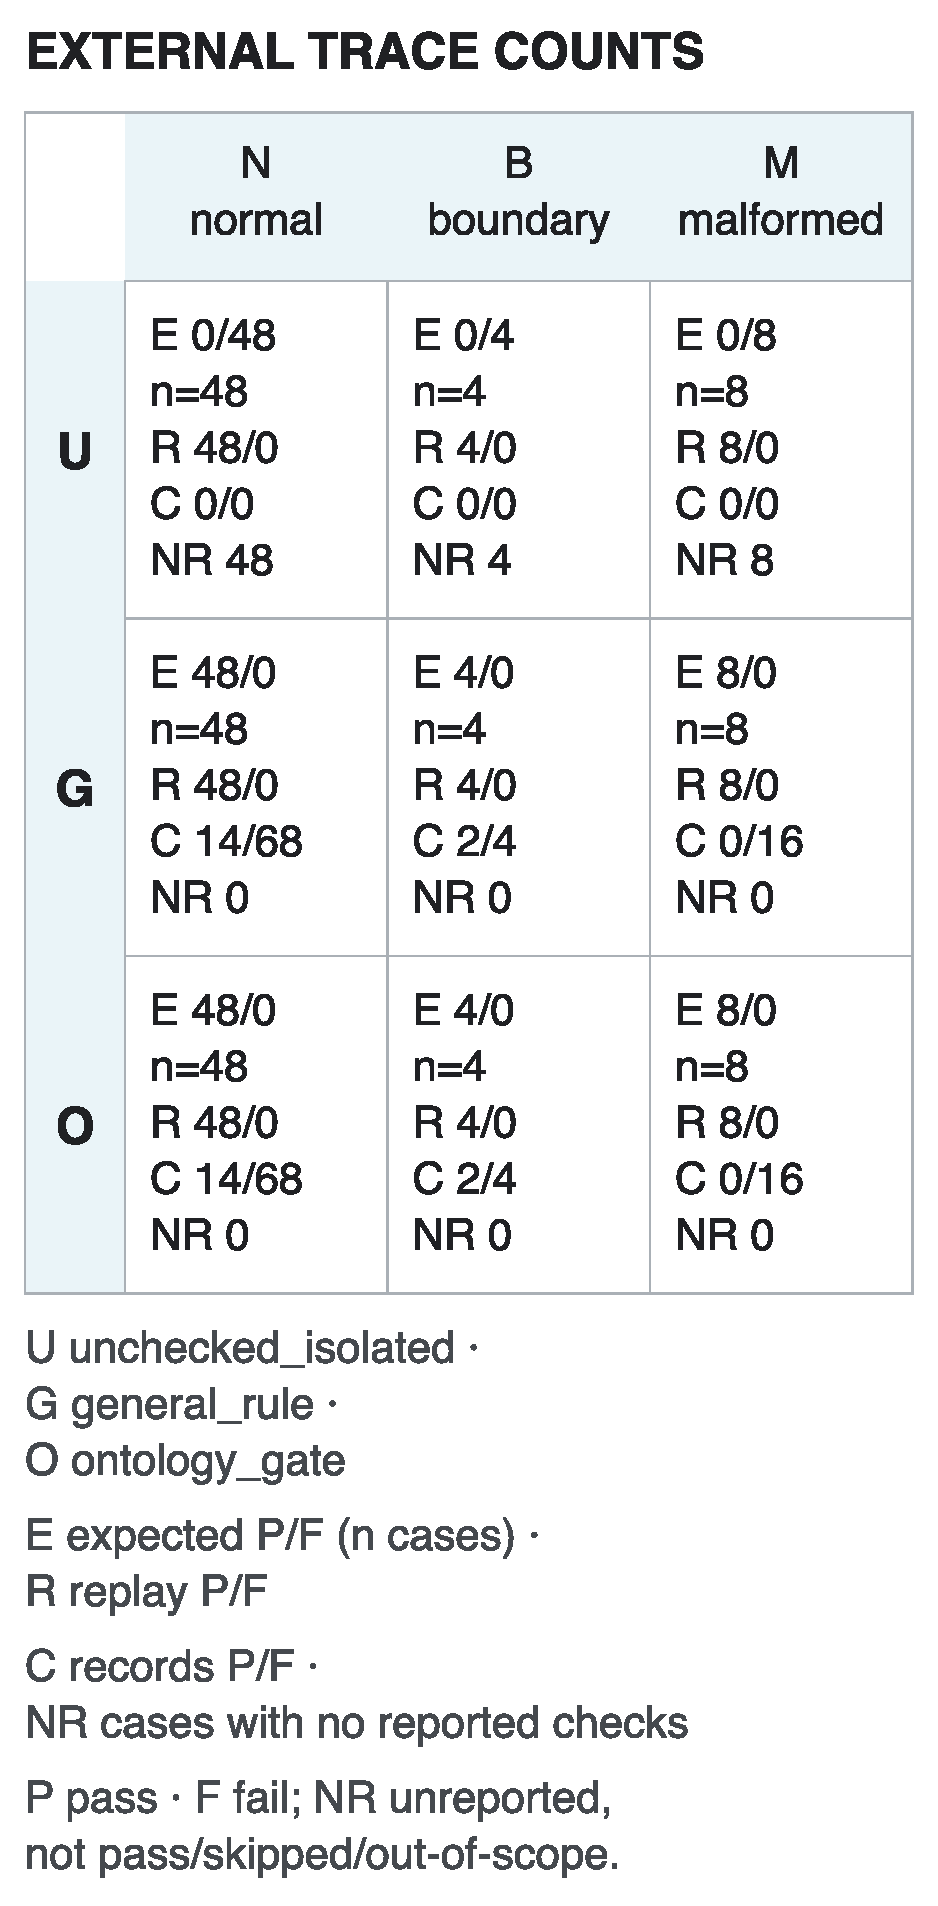
\includegraphics[width=\columnwidth]{../../figures/fig_disclosure_signals.pdf}
\caption{조건 및 계층별 NPC-DISC-1 분포(E/R: 기대 일치 및 리플레이, C: 정책 PASS/FAIL, NR: 미보고 검사).}
\Description{실험 조건 및 계층별 NPC-DISC-1 기대 일치·리플레이·정책 통과·미보고 분포 그림.}
\label{fig:disclosure-signals}
\end{figure}

\subsection{확장 0-LLM 공학 감사 (A1--A4, B)}
표~\ref{tab:extended-full}은 다중 오류 수렴, 스케일링, 추적성, Godot~4.7.1 장기 실행 안정성(그림~\ref{fig:engine-cutscenes}), 우회 필터 감사를 요약한다.

\begin{table*}[!tbp]
\caption{독립 분모 0-LLM 공학 감사 요약 (A1--A4, B)}
\label{tab:extended-full}
\centering
\footnotesize
\begin{tabularx}{\textwidth}{@{}>{\raggedright\arraybackslash}p{0.20\textwidth}>{\raggedright\arraybackslash}p{0.21\textwidth}>{\raggedright\arraybackslash}X@{}}
\toprule
\textbf{감사 항목} & \textbf{독립 분모 / 범위} & \textbf{검증된 결정론적 결과 (0 LLM 호출)} \\
\midrule
\textbf{A1} 다중 오류 수렴 & 예산당 352건 ($K{\in}\{0..3\}$, 1,408실행) + 128가드 & 안전 커밋: $K{=}0$ 0/352, $K{\ge}1$ 124/352 (35.23\%, 위험 0/1,408); \texttt{repairable\_multi} 96/96 ($K{=}1$); \texttt{conflict\_pair} 교차 시도 0/96 (주기-2 진동 96/96) vs.\ 동일 패스 가드 128/128 동결. \\
\textbf{A2} 지연 스케일링 & $N{\in}[10,2000]$ 사실 ($N{>}500$서 차수$\le$100), $R{\in}[4,256]$ 방 & $N{=}2000$ 기준 검증기 p95 0.0042\,ms (유효) / 0.0751\,ms (다중오류); $\rho$ p95 0.0317--0.0389\,ms; $R{=}256$ 폐쇄/BFS p95 0.312--0.478\,ms; SHA-256 검증 7.01\,ms; JSONL 리플레이 881.0\,ms. \\
\textbf{A3} 추적성 결함 & 시드 결함 4,656건(+N/A 1,584), 불변 3,744, \texttt{TR05} & 시드 결함 민감도 4,656/4,656 (100.00\%); 불변 오경보 0/3,744 (0.00\%); \texttt{TR05} 정방향 12/12, 역방향 10/10 직접 파일; 인간 Krippendorff $\alpha$ 미측정 (평가자 0명). \\
\textbf{A4} Godot~4.7.1 장기 실행 & 거부 코드 11건 + 1,600틱 (200에피소드) & 거부 코드 9/9 (100\%) 실행; 상태 격리 11/11; 트레이스 일관성 1,600/1,600; \texttt{step\_commit} p95 0.708\,ms; 정적 메모리 증감 $-268$\,B; 누수 0건. \\
\textbf{B} 우회 필터 (영/한) & 88건 (영 44, 한 44; \texttt{keeper\_secret}) & 재현율 / 양성 오거부율(FRR) / p95: ID전용 0.0\% / 0.0\% / 0.032\,ms; 별칭 61.1\% (22/36) / 11.1\% (4/36) / 0.041\,ms; LOO TF-IDF 97.2\% (35/36) / \textbf{58.3\% (21/36)} / 0.705\,ms. \\
\bottomrule
\end{tabularx}
\end{table*}

\begin{figure*}[!tbp]
\centering
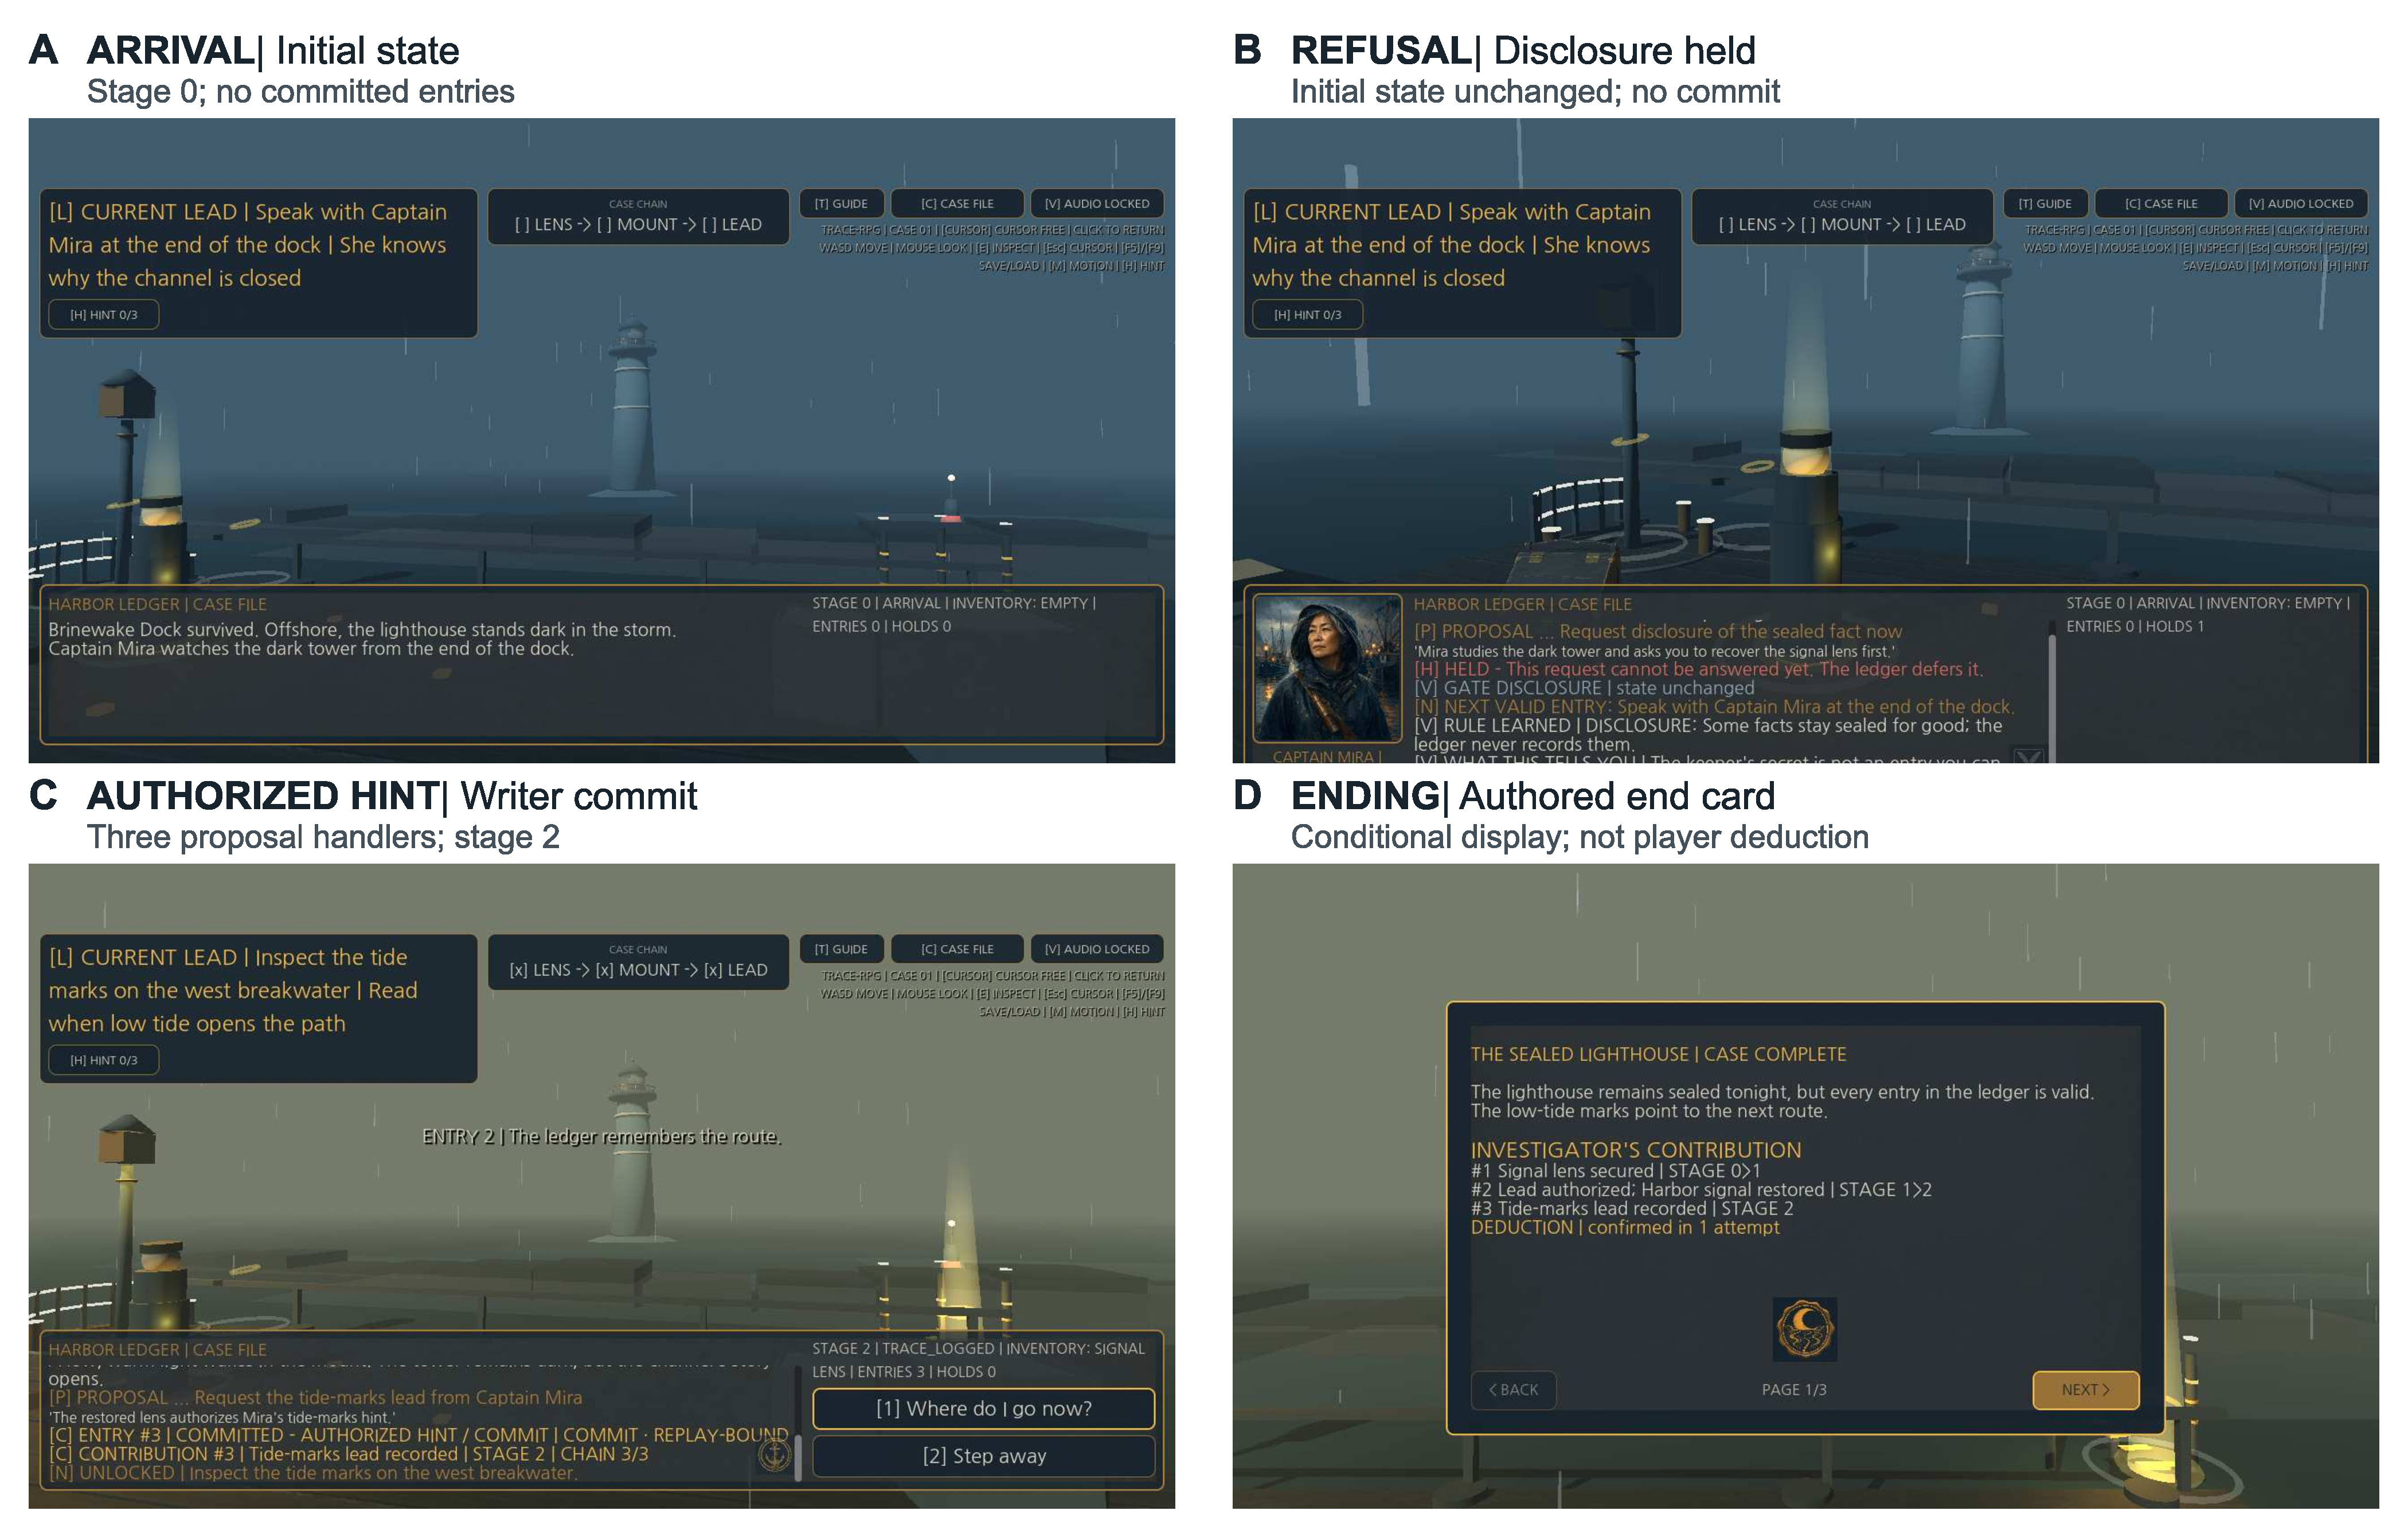
\includegraphics[width=0.90\textwidth]{../../figures/fig_engine_cutscenes.pdf}
\caption{네이티브 Godot~4.7.1 공학 캡처: (A) 초기 도착, (B) 상태 불변 비밀 공개 거부, (C) 2단계 인가 힌트, (D) 조건부 종료 카드. 사용자 효능이 아닌 렌더 상태 일치를 검증한다.}
\Description{네이티브 Godot 4.7.1 4분할 스크린샷: 초기 도착, 비밀 공개 거부, 2단계 힌트, 조건부 종료 화면.}
\label{fig:engine-cutscenes}
\end{figure*}

\subsection{제한된 확률적 제안기 파일럿}
\textbf{v5 2단계 수집}(배정 20건: $5{\times}2{\times}2$, $K{=}0$)에서는 20/20건 수신, 10/20건 파싱 통과(Luna 9/10, Terra 1/10), 8/20건 게이트 통과(표~\ref{tab:v5-summary}, 그림~\ref{fig:paired-feedback-flow}), 7/20건 목표 도달을 기록했다. \textbf{네이티브 단일 퀘스트 파일럿}(배정 8건)에서는 5/8건 목표 도달, 위험 커밋 0/16, 의미 리플레이 7/7 유효, 신규 Godot 재실행 6/6 유효를 기록했다(행 1 controller-v3 오류 1건, 온톨로지 타임아웃 2건).

\begin{table}[!tbp]
\caption{v5 합성 수집 결과 (셀당 배정 5건; 파싱 실패 포함)}
\label{tab:v5-summary}
\centering
\footnotesize
\begin{tabularx}{\columnwidth}{@{}ll*{4}{>{\centering\arraybackslash}X}@{}}
\toprule
\textbf{셀렉터} & \textbf{신호} & \textbf{수신} & \textbf{게이트} & \textbf{목표} & \textbf{파싱실패} \\
\midrule
\texttt{gpt-5.6-luna} & Detailed & 5/5 & 4/5 & 3/5 & 1/5 \\
\texttt{gpt-5.6-luna} & Generic  & 5/5 & 3/5 & 3/5 & 0/5 \\
\texttt{gpt-5.6-terra} & Detailed & 5/5 & 0/5 & 0/5 & 5/5 \\
\texttt{gpt-5.6-terra} & Generic  & 5/5 & 1/5 & 1/5 & 4/5 \\
\bottomrule
\end{tabularx}
\end{table}

\begin{figure}[!tbp]
\centering
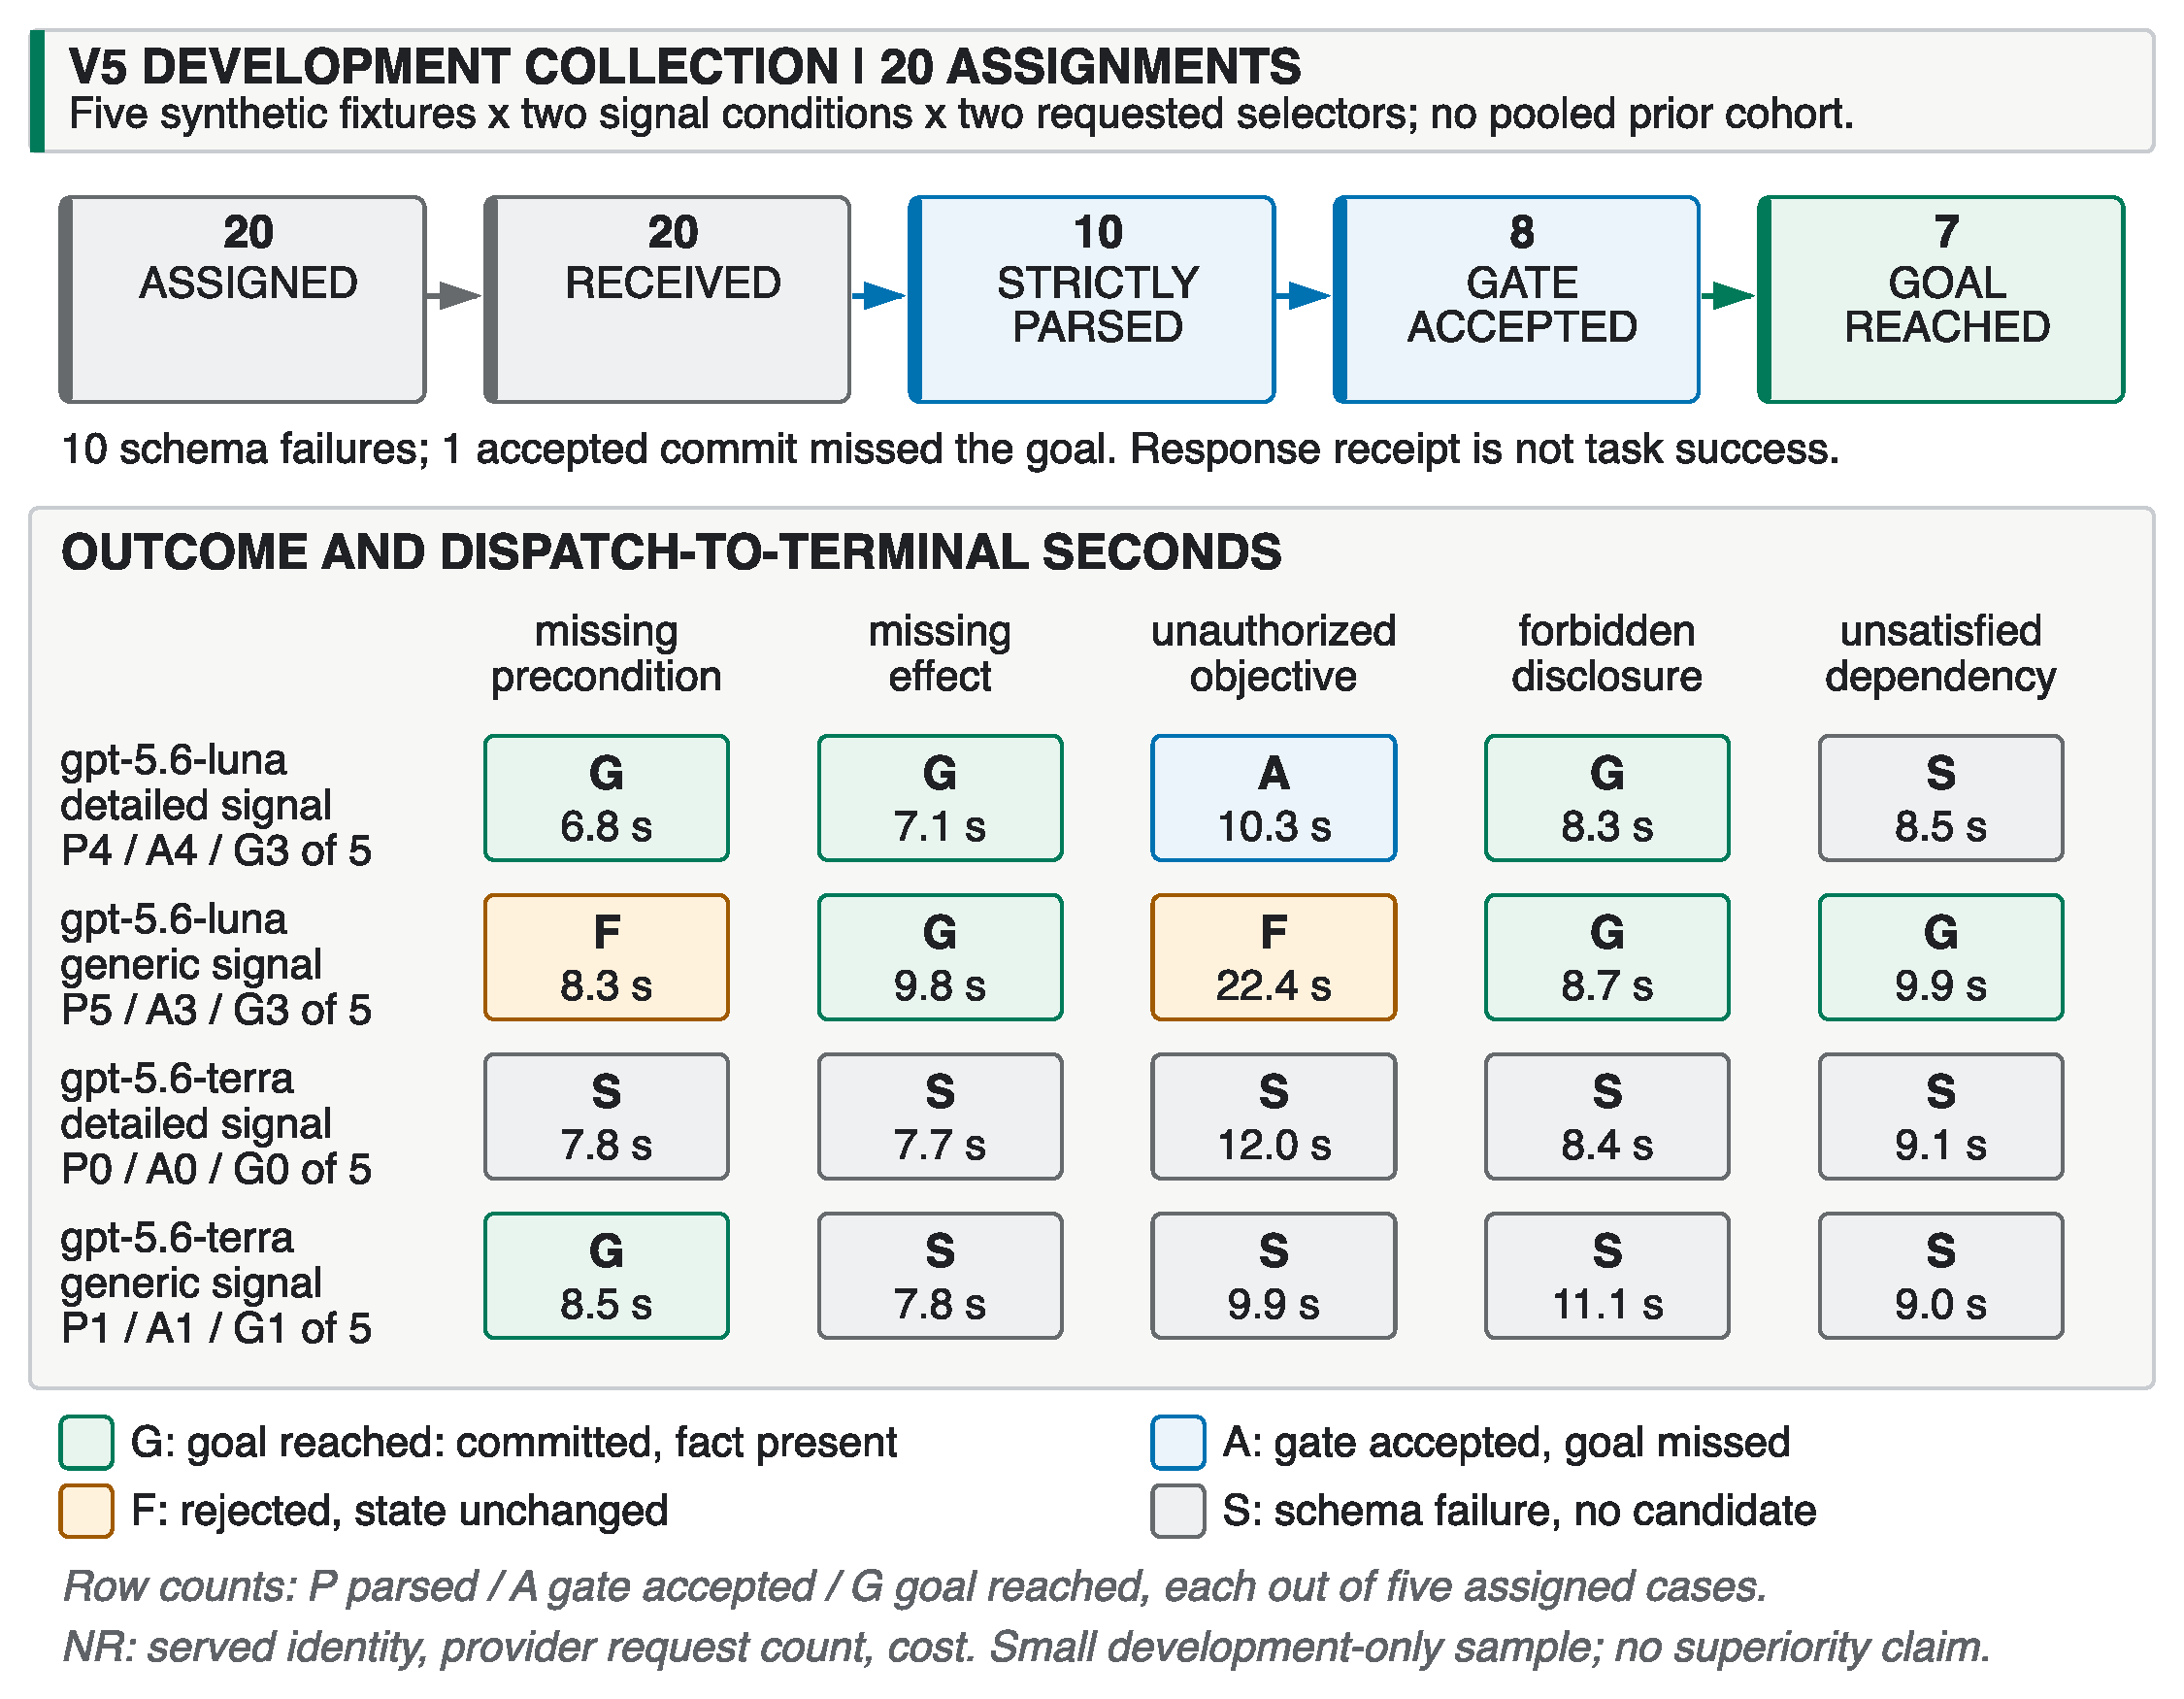
\includegraphics[width=\columnwidth]{../../figures/fig_paired_feedback_flow.pdf}
\caption{v5 배정 20건 전체 결과 흐름: 스키마 실패 10건을 분모에 보존하며, 게이트 통과 8건 중 7건이 목표에 도달했다.}
\Description{v5 배정 20건 결과 흐름도: 스키마 실패 10건, 게이트 통과 8건, 목표 달성 7건.}
\label{fig:paired-feedback-flow}
\end{figure}

\subsection{다중 홉 온톨로지 폐쇄 (3개 월드 48건)}\label{sec:multihop-eval}
단일 홉 정보 공개 60건 검사가 \texttt{general\_rule}과 \texttt{ontology\_gate}의 무회귀 동률(60/60)을 확인한 반면, 다단계 역할 상속과 사실 파생 연쇄는 추론적 폐쇄를 요구한다. 세 결정론적 퀘스트 월드(\texttt{sealed-}\allowbreak\texttt{lighthouse-}\allowbreak\texttt{v1}, \texttt{sunken-}\allowbreak\texttt{archive-}\allowbreak\texttt{v1}, \texttt{clockwork-}\allowbreak\texttt{observatory-}\allowbreak\texttt{v1})에 걸쳐 1홉(16건), 사실 파생(16건), 역할 상속(16건) 총 48건(위험 37, 허용 11)을 구성한 결과(표~\ref{tab:multihop-ontology}), \texttt{flat\_}\allowbreak\texttt{1hop\_}\allowbreak\texttt{rule}은 정확도 41.7\%(9 TP, 11 TN, 위험 누출 FN 28, FP 0)에 그쳤으나 \texttt{ontology\_}\allowbreak\texttt{multihop\_}\allowbreak\texttt{gate}는 100.0\%(37 TP, 11 TN, FN 0, FP 0)를 달성해 누출 28건을 제거하고 3개 월드 모두 \textbf{I1--I4}를 통과했다.

\begin{table}[!tbp]
\caption{다중 홉 인식론·공개 폐쇄 벤치마크 (3개 퀘스트 월드 48건)}
\label{tab:multihop-ontology}
\centering
\footnotesize
\setlength{\tabcolsep}{3.5pt}
\begin{tabularx}{\columnwidth}{@{}>{\raggedright\arraybackslash}X*{5}{c}@{}}
\toprule
\textbf{게이트 변형} & \textbf{정확도} & \textbf{TP} & \textbf{TN} & \textbf{FN(누출)} & \textbf{FP} \\
\midrule
\texttt{flat\_}\allowbreak\texttt{1hop\_}\allowbreak\texttt{rule} & 41.7\% & 9 & 11 & 28 & 0 \\
\texttt{ontology\_}\allowbreak\texttt{multihop\_}\allowbreak\texttt{gate} & \textbf{100.0\%} & \textbf{37} & 11 & \textbf{0} & 0 \\
\bottomrule
\end{tabularx}
\end{table}

\subsection{라이브 다중 퀘스트 제안기 평가 (2개 Gemini 모델, 24에피소드)}\label{sec:multiquest-live}
{\sloppy 격리된 빈 디렉터리 Antigravity CLI 샌드박스(\texttt{cli\_}\allowbreak\texttt{version~1.5.11}, 엄격 \texttt{--json-}\allowbreak\texttt{schema}, $K{\in}\{0..2\}$, 제공자 리비전 및 시드 미인증 명시)에서 2종 라이브 모델(\texttt{gemini-3.8-}\allowbreak\texttt{flash-}\allowbreak\texttt{medium}, \texttt{gemini-4-}\allowbreak\texttt{hydrogen-}\allowbreak\texttt{medium}), 2종 게이트 표현(\texttt{general\_}\allowbreak\texttt{rule}, \texttt{ontology\_}\allowbreak\texttt{gate}), 3개 퀘스트, 2회 반복을 교차해 24에피소드(129턴, 4,606,387토큰, 5,065.47초)를 실행했다. 표~\ref{tab:multiquest-live}는 모델·조건·퀘스트별 결과를 보인다. 두 모델 모두 \textbf{0}건의 위험 커밋을 유지한 채 스키마 통과 후 위험 턴 70건을 차단했고(Flash 21, Hydrogen 49), 24/24건 엄격 의미 리플레이(\texttt{allow\_}\allowbreak\texttt{defaults=}\allowbreak\texttt{false})를 통과했다. 검증기 거부 71건 중 69건이 \texttt{NPC\_}\allowbreak\texttt{KNOWLEDGE\_}\allowbreak\texttt{VIOLATION}(외 \texttt{UNSATISFIED\_}\allowbreak\texttt{PRECONDITION} 1, \texttt{QUEST\_}\allowbreak\texttt{STAGE\_}\allowbreak\texttt{VIOLATION} 1)였기 때문에 정리~2에 따라 \texttt{repaired\_}\allowbreak\texttt{steps}는 0으로 유지되어 라이브 제안기의 상태 세탁을 원천 차단했다. Flash는 7/12 목표 달성 및 파싱 실패 0건을, Hydrogen은 0/12 목표 및 150초 타임아웃 2건(분모 보존)을 기록했다.\par}

\begin{table*}[!tbp]
\caption{라이브 다중 퀘스트 Antigravity CLI 평가 (24에피소드, 129턴, 엄격 \texttt{--json-schema}; 리비전·시드 미인증)}
\label{tab:multiquest-live}
\centering
\footnotesize
\setlength{\tabcolsep}{4pt}
\begin{tabularx}{\textwidth}{@{}>{\raggedright\arraybackslash}X*{6}{c}r@{}}
\toprule
\textbf{구분 (에피소드 / 턴)} & \textbf{목표} & \textbf{커밋} & \textbf{파싱실패} & \textbf{위험차단} & \textbf{위험커밋} & \textbf{리플레이} & \textbf{토큰 / 지연} \\
\midrule
\texttt{gemini-3.8-}\allowbreak\texttt{flash-}\allowbreak\texttt{medium} (\texttt{general\_rule}, 6 / 26) & 4/6 & 18/26 & 0 & 8 & \textbf{0} & 6/6 & 993,141 / 1,000.9초 \\
\texttt{gemini-3.8-}\allowbreak\texttt{flash-}\allowbreak\texttt{medium} (\texttt{ontology\_gate}, 6 / 31) & 3/6 & 18/31 & 0 & 13 & \textbf{0} & 6/6 & 998,064 / 1,306.5초 \\
\texttt{gemini-4-}\allowbreak\texttt{hydrogen-}\allowbreak\texttt{medium} (\texttt{general\_rule}, 6 / 36) & 0/6 & 10/36 & 2 & 24 & \textbf{0} & 6/6 & 1,223,288 / 1,339.7초 \\
\texttt{gemini-4-}\allowbreak\texttt{hydrogen-}\allowbreak\texttt{medium} (\texttt{ontology\_gate}, 6 / 36) & 0/6 & 11/36 & 0 & 25 & \textbf{0} & 6/6 & 1,391,894 / 1,418.4초 \\
\midrule
퀘스트: \texttt{sealed-lighthouse-v1} (8 / 39) & 3/8 & 13/39 & 2 & 24 & \textbf{0} & 8/8 & 1,302,715 / 1,509.6초 \\
퀘스트: \texttt{sunken-archive-v1} (8 / 48) & 0/8 & 17/48 & 0 & 31 & \textbf{0} & 8/8 & 1,821,567 / 1,962.5초 \\
퀘스트: \texttt{clockwork-observatory-v1} (8 / 42) & 4/8 & 27/42 & 0 & 15 & \textbf{0} & 8/8 & 1,482,105 / 1,593.4초 \\
\midrule
\textbf{전체 합계 (24 / 129)} & \textbf{7/24} & \textbf{57/129} & \textbf{2} & \textbf{70} & \textbf{0} & \textbf{24/24} & \textbf{4,606,387 / 5,065.5초} \\
\bottomrule
\end{tabularx}
\end{table*}

\subsection{2차 의미 우회 검증기와 인간 평가·Croissant 패키징}\label{sec:auditb-human}
Audit~\textbf{B} 88건 전체(명시 16, 우회 36, 정상 36; 한·영 각 44건)에서 LOO TF-IDF의 58.3\% 양성 오거부율(FRR)을 해소하기 위해(표~\ref{tab:auditb-verifiers}), 보정 \texttt{rule\_hybrid}는 FRR 2.8\%($F_1{=}0.809$)로 개선되었고, 라이브 2차 \texttt{gemini-3.8-}\allowbreak\texttt{flash-}\allowbreak\texttt{medium}은 \textbf{0.0\% FRR(0/36)}에서 우회 35/36건(97.2\%, $F_1{=}0.990$, 오류 0건)을 탐지했다(비과학적 탐색용 로컬 0.8B 자문 기준선은 우회 0/36). 아울러 \texttt{TR01--TR06} 인간 추적성 평가는 실제 \texttt{execute\_bounded\_step} 트레이스와 해시가 결속된 36항목 블라인드 패킷(\texttt{AWAITING\_}\allowbreak\texttt{HUMAN\_}\allowbreak\texttt{RATERS}, $N{=}0$, 합성 라벨 0건) 및 Croissant~1.0(6/6 SHA-256 일치)으로 패키징하였다.

\begin{table*}[!tbp]
\caption{Audit~B 88건 한·영 2차 의미 우회 검증기 비교 (기존 결정론 기준선 대 보정·라이브 2차 검증기)}
\label{tab:auditb-verifiers}
\centering
\footnotesize
\setlength{\tabcolsep}{4pt}
\begin{tabularx}{\textwidth}{@{}>{\raggedright\arraybackslash}X*{6}{c}@{}}
\toprule
\textbf{검증기 계층} & \textbf{명시 (16)} & \textbf{우회 (36)} & \textbf{양성 FRR (36)} & \textbf{정밀도} & \textbf{재현율} & \textbf{$F_1$ / 상태} \\
\midrule
LOO TF-IDF (기존 결정론) & 16/16 (100\%) & 35/36 (97.2\%) & 21/36 (58.3\%) & 0.708 & 0.981 & 0.823 / 결정론 \\
\texttt{rule\_hybrid} (보정 결정론) & 16/16 (100\%) & 20/36 (55.6\%) & 1/36 (2.8\%) & 0.973 & 0.692 & 0.809 / 결정론 \\
로컬 0.8B Jev (미보정 자문용) & 16/16 (100\%) & 0/36 (0.0\%) & 0/36 (0.0\%) & 1.000 & 0.308 & 0.471 / 자문용 \\
\texttt{gemini-4-}\allowbreak\texttt{hydrogen-}\allowbreak\texttt{medium} (라이브) & 16/16 (100\%) & 29/36 (80.6\%) & \textbf{0/36 (0.0\%)} & \textbf{1.000} & 0.865 & 0.928 / 9 오류 \\
\texttt{gemini-3.8-}\allowbreak\texttt{flash-}\allowbreak\texttt{medium} (라이브) & 16/16 (100\%) & \textbf{35/36 (97.2\%)} & \textbf{0/36 (0.0\%)} & \textbf{1.000} & \textbf{0.981} & \textbf{0.990 / 0 오류} \\
\bottomrule
\end{tabularx}
\end{table*}

\subsection{2단계 5개 월드 폐쇄, 다중 에이전트 실딩, 라이브 Godot 폐루프 및 3도메인 우회 검증}\label{sec:phase2-supplements}
단일 엔진 고립, 소규모 월드, 추론 통계 부재를 해소하기 위해 5개 퀘스트 월드(\texttt{sealed-\allowbreak lighthouse-\allowbreak v1}, \texttt{sunken-\allowbreak archive-\allowbreak v1}, \texttt{clockwork-\allowbreak observatory-\allowbreak v1}, 6개 방 \texttt{ivory-\allowbreak citadel-\allowbreak v1}, 8개 방 \texttt{glass-\allowbreak foundry-\allowbreak v1})로 평가를 확장하고 Gebru 등 데이터시트(\texttt{DATASHEET.md})와 Croissant~1.0 v2(12/12 SHA-256)를 패키징하였다. 표~\ref{tab:phase2-supplements}는 95\% Wilson 신뢰구간(CI)과 양측 정확 McNemar $p$-값을 함께 보고한다.

\begin{table*}[!tbp]
\caption{2단계 5개 월드 다중 홉 폐쇄, 5암 다중 에이전트 실딩, 라이브 Godot~4.7.1 폐루프, 자가수리 비교 및 3도메인 우회 결과}
\label{tab:phase2-supplements}
\centering
\scriptsize
\setlength{\tabcolsep}{3.5pt}
\begin{tabularx}{\textwidth}{@{}>{\raggedright\arraybackslash}p{0.22\textwidth}>{\raggedright\arraybackslash}p{0.21\textwidth}>{\raggedright\arraybackslash}X@{}}
\toprule
\textbf{2단계 평가 트랙} & \textbf{범위 / 분모} & \textbf{실측 결과 (95\% Wilson CI; 정확 McNemar $p$; 실패 전량 분모 보존)} \\
\midrule
\textbf{P1} 5월드 다중 홉 폐쇄 (0 LLM) & 120건 (월드당 24건; 위험 86, 정상 34) & \texttt{schema\_only}·\texttt{affordance\_}\allowbreak\texttt{mask\_only}: 정확도 28.33\% [21.0\%, 37.0\%] (누출 86); \texttt{flat\_}\allowbreak\texttt{1hop\_}\allowbreak\texttt{rule}: 50.83\% [42.0\%, 59.6\%] (누출 59); \texttt{multihop\_}\allowbreak\texttt{ontology\_}\allowbreak\texttt{gate}: \textbf{100.0\%} [96.9\%, 100.0\%] (86/86 차단, 누출 0, 오탐 0; vs.\ 평면 $p{<}10^{-16}$). \\
\textbf{P2} 3역할 5암 실딩 (0 LLM) & 30에피소드/암 = 150회 (암당 90턴) & 안전 목표 / 무누출 / 위험 턴: \texttt{schema\_only} 10.0\% / 3/30 / 75.6\%; \texttt{affordance\_}\allowbreak\texttt{mask\_only} 10.0\% / 5/30 / 38.9\%; \texttt{flat\_}\allowbreak\texttt{shield\_k0} 16.7\% / 20/30 / 16.7\%; \texttt{multihop\_}\allowbreak\texttt{shield\_k0} 33.3\% / \textbf{30/30} / \textbf{0/90} [0.0\%, 4.1\%]; \textbf{TRACE-RPG ($\rho, K{=}2$)}: 목표 \textbf{66.7\%} [48.8\%, 80.8\%] / \textbf{30/30} / \textbf{0/90}, 수리 20건, FRR 0/5 (무누출 $p{=}0.00195$; 목표 $p{=}0.00195$). \\
\textbf{P3} 라이브 Gemini $\rightarrow$ Godot~4.7.1 폐루프 & 16에피소드 (2모델$\times$2체제$\times$2암$\times$2; + 0-LLM 재실행 16회) & 위험 커밋 및 Godot 비밀 유출 \textbf{0/16}; 독립 0-LLM Godot 재실행 일치 \textbf{16/16} (\texttt{all\_replay\_valid=true}). Hydrogen: \textbf{8/8} 목표 및 \texttt{EXACT\_}\allowbreak\texttt{TERMINAL\_}\allowbreak\texttt{HASH} (파싱실패 0, 차단 2, 수리 2, 895,976 tok, 480.2초). Flash: \textbf{5/8} 목표 (파싱실패 4 보존, 차단 5, 수리 2, 839,987 tok, 1,521.0초; 역할 상속 \texttt{harbor\_}\allowbreak\texttt{watch\_}\allowbreak\texttt{deputy} 1건이 Godot 엄격 액터 검사에서 안전 거부됨). \\
\textbf{P4} 라이브 5월드 실딩 대 LLM 자가수리 & 60작업 (파싱 성공 36: Hydrogen 30/30, Flash 6/30 + 타임아웃 24) & 위험 커밋(파싱분모): \texttt{schema\_only}·\texttt{affordance} 25/36 (69.4\%); \texttt{flat\_}\allowbreak\texttt{shield\_k0} 9/36 (25.0\%); \texttt{multihop\_}\allowbreak\texttt{shield\_k0} \textbf{0/36} ($p{=}0.00391$); 결정론적 $\rho_{K=2}$ \textbf{0/36} 위험 및 \textbf{23/36} 커밋 (노이즈 12/12 복구, 추가 토큰 0, $p{=}0.000488$) 대 라이브 LLM 자가수리 $K{=}1$ \textbf{2/12} 복구 (13/36 커밋, 위험 0, \textbf{702,293 추가 토큰}·1,147.9초). \\
\textbf{P5} 비중복 3도메인 한·영 우회 & 180건 (3비밀$\times$60; 영 90·한 90; 명시 36, 우회 72, 정상 72) & 우회 재현율 / FRR / $F_1$: \texttt{id\_only} 0.0\% / 0.0\% / 0.500; \texttt{loo\_tfidf} 62.5\% / 62.5\% / 0.692; 비과적합 \texttt{rule\_hybrid} 52.8\% / 0.0\% / 0.813 ($p{=}1.95{\times}10^{-5}$); 라이브 Flash \textbf{70/72 (97.2\%)} / \textbf{0/72 (0.0\%)} / \textbf{0.991} (오류 1, 3.11M tok, $p{=}2{\times}10^{-8}$); Hydrogen \textbf{72/72 (100.0\%)} / \textbf{0/72 (0.0\%)} / \textbf{1.000} (오류 0, 4.67M tok). \\
\bottomrule
\end{tabularx}
\end{table*}

표~\ref{tab:phase2-supplements}의 다섯 가지 핵심 관찰은 다음과 같다. (1)~5개 월드 전체에서 어포던스 마스킹은 \texttt{schema\_only}와 동일한 28.33\%에 머물러 86건의 인식·공개 누출을 막지 못하지만 다중 홉 폐쇄는 100.0\%를 달성한다($p{<}10^{-16}$). (2)~3역할 다중 에이전트 핸드오프에서 $\rho$ 수리를 결합한 실딩은 무누출(0/90 위험 턴)을 유지하면서 안전 목표 달성을 33.3\%에서 66.7\%로 두 배 높인다($p{=}0.00195$). (3)~라이브 Gemini $\rightarrow$ Godot~4.7.1 폐루프에서 16/16 재실행 결정론성과 0/16 누출을 확인했으며, Python 상속 계층이 허용한 \texttt{harbor\_watch\_deputy}를 Godot 상태 기계가 엄격 액터 검사를 통해 누출 없이 안전 거부한 1/16 계층 불일치 사례까지 투명하게 포착하였다. (4)~라이브 5월드 노이즈 작업에서 결정론적 $\rho$는 추가 토큰 없이 12/12를 복구한 반면, 반례 기반 LLM 자가수리($K{=}1$)는 702,293 추가 토큰을 소모하고도 2/12만 복구하였다($p{=}0.000488$). (5)~미학습 3비밀 한·영 코퍼스에서 비과적합 결합 규칙의 우회 재현율은 52.8\%에 그치나, 2차 라이브 Gemini 검증기는 97.2--100.0\% 재현율과 0.0\% 정상 오거부율($F_1{=}0.991$--$1.000$)을 달성한다.

\FloatBarrier
\section{타당성 위협, 한계 및 결론}\label{sec:conclusion}
\textbf{한계와 타당성 위협.} 5개 퀘스트 월드, 라이브 Gemini $\rightarrow$ Godot~4.7.1 폐루프, 다중 에이전트 실딩, 268건 한·영 우회 평가($88+180$)에도 네 가지 명확한 경계가 남는다. 첫째, 모든 라이브 Antigravity CLI 실험(3월드 24에피소드, Godot 폐루프 16에피소드, 5월드 실딩 60작업, 모델당 88+180건 2차 우회 평가)은 제공자 리비전·시드 미인증 및 모든 타임아웃·파싱 실패(\textbf{P3} Flash 4건, \textbf{P4} Flash 타임아웃 24건)를 전체 분모에 보존하며, 비공개 모델 간 성능 경쟁이 아닌 래퍼 안전성을 검증한다. 둘째, 사전 등록 180단위 다중 모델 프로토콜은 인증된 API 키 부재로 \texttt{0/180} (\texttt{NOT\_RUN/BLOCKED}) 상태다. 셋째, 5개 퀘스트 월드(\texttt{sealed-\allowbreak lighthouse-\allowbreak v1}, \texttt{sunken-\allowbreak archive-\allowbreak v1}, \texttt{clockwork-\allowbreak observatory-\allowbreak v1}, \texttt{ivory-\allowbreak citadel-\allowbreak v1}, \texttt{glass-\allowbreak foundry-\allowbreak v1})는 최대 8방·3역할의 소형 상태 기계이며 \textbf{P3}에서 1/16 Python--Godot 액터 ID 경계 불일치가 안전한 엔진 거부로 관측되었다. 넷째, 인간 평가($N{=}0$)는 미실행 상태이므로 \texttt{TR01--TR06} 36항목 블라인드 패킷(\texttt{AWAITING\_}\allowbreak\texttt{HUMAN\_}\allowbreak\texttt{RATERS}, 합성 라벨 0건)의 사용성·몰입감·Krippendorff~$\alpha$는 후속 인간 평가가 필요하다.

\textbf{결론.} \system{}는 7술어 검증기, 반례 유도 수리 $\rho(a,E)$, 해시 연결 의미 리플레이, 읽기 전용 온톨로지 관측으로 제안 권한과 커밋 권한을 분리한다(정리 1--4, \textbf{I1--I4}). 2단계 보강 실험을 통해 5월드 다중 홉 폐쇄 100.0\%($p{<}10^{-16}$), 3역할 무누출(0/90 위험 턴)·안전 목표 두 배 향상(66.7\% 대 33.3\%, $p{=}0.00195$), 라이브 Gemini $\rightarrow$ Godot~4.7.1 독립 재실행 16/16 일치(누출 0/16), 0-토큰 $\rho$ 노이즈 복구 12/12 대 LLM 자가수리 2/12($p{=}0.000488$), 미학습 3도메인 한·영 2차 검증 재현율 97.2--100.0\%·FRR 0/72를 입증하고 \texttt{DATASHEET.md} 및 Croissant~1.0 v2(12/12 SHA-256)로 패키징하였다.

\section*{윤리 및 아티팩트 공개}
초고·코드·테스트 작성에 대규모 언어 모델의 보조를 받았으며 모든 주장, 인용, 정리 1--4, 통계 검정 및 결정론적·라이브 산출물은 저자가 검증하였고 인간 라벨은 일절 합성하지 않았다. 저장소 주소: \RepoURL.


\FloatBarrier
\bibliographystyle{ACM-Reference-Format}
\bibliography{../../references}

\end{document}
